\documentclass[letterpaper,12pt]{article}

\usepackage{ge05}
\usepackage{comment}
\usepackage{booktabs}
\usepackage[dvipdfm]{hyperref}
\urlstyle{rm}   % change fonts for url's (from Chad Jones)
\hypersetup{
    colorlinks=true,        % kills boxes
    allcolors=blue,
    pdfsubject={NYU Stern course GB 2303, Global Economy},
    pdfauthor={Dave Backus @ NYU},
    pdfstartview={FitH},
    pdfpagemode={UseNone},
%    pdfnewwindow=true,      % links in new window
%    linkcolor=blue,         % color of internal links
%    citecolor=blue,         % color of links to bibliography
%    filecolor=blue,         % color of file links
%    urlcolor=blue           % color of external links
% see:  http://www.tug.org/applications/hyperref/manual.html
}

\newcommand{\GDP}{\mbox{\em GDP\/}}
\newcommand{\NDP}{\mbox{\em NDP\/}}
\newcommand{\GNP}{\mbox{\em GNP\/}}
\newcommand{\NX}{\mbox{\em NX\/}}
\newcommand{\NY}{\mbox{\em NY\/}}
\newcommand{\CA}{\mbox{\em CA\/}}
\newcommand{\NFA}{\mbox{\em NFA\/}}
\newcommand{\Def}{\mbox{\em Def\/}}
\newcommand{\CPI}{\mbox{\em CPI\/}}

\def\ClassName{The Global Economy}
\def\Category{Class Notes}
\def\HeadName{Policy in the AS/AD Model}

\begin{document}
\thispagestyle{empty}%
\Head

\centerline{\large \bf \HeadName}%
\centerline{Revised: \today}

\bigskip
We've seen that aggregate demand and supply can shift on their own or,
sometimes, as a result of changes in policy,
including monetary policy.
But what policy changes are called for?
Should we always shift the aggregate demand curve to maintain
low inflation?  High output?
Are these two objectives in conflict?
The short answer:
we should respond differently to changes in supply and demand.


\subsubsection*{Objectives of policy}

The traditional guide to policy is the invisible hand:
if markets work well, then we simply leave them to do their job.
If not, we may act to facilitate their operation.
In the aggregate demand and supply framework,
the idea is that the long-run aggregate supply curve
is where the uninhibited operation of markets would lead us.
In the short run, sticky wages (or other market imperfection)
may resist, but that's
where the invisible hand would direct us.
One consequence:   there's no
compelling reason to change aggregate demand
to increase output beyond its long-run equilibrium value.
We might be able to do it, but it won't make us better off.
In a sense, we will have tricked people into working more than they
want,
typically by reducing their real wages through inflation.

The first objective of policy, then,
is to get output as near as possible to
the level associated with the long-run
aggregate supply curve AS$^*$.
This is important enough a concept that people have given it
lots of names:  potential output, full employment output, and so on.
We'll call it {\it potential output\/}, with the understanding that it's
the long-run equilibrium, not an upper bound.
The {\it output gap\/} is a related concept:
the difference between actual and potential output.
In practice, potential output is a little slippery,
because the long-run aggregate supply curve
isn't something we observe.
We have a variety of ways of estimating potential output,
ranging from the complex (the Fed's methodology, described
in a link listed at the end of these notes) to
the pragmatic (a smooth trend line drawn through actual output).

%%%%%%%%%%%%%%%%%%%%%%%%%%%%%%%%%%%%%%%%%%%%%%%%%%%%%%%%%%%%%%%%%%%%%%%%%%%%
%  Supply and demand diagram
\begin{figure}[h!]
%
\begin{center}
\setlength{\unitlength}{0.075em}
\begin{picture}(250,200)(0,0)
%\footnotesize
\thicklines

% horizontal axis
\put(-30,0){\vector(1,0){300}}
\put(255,-16){$Y$}
\put(142,-16){$Y^*$}

% vertical axis
\put(0,-20){\vector(0,1){200}}
\put(-15,155){$P$}

% demand
\put(25,165){\line(4,-3){200}}\put(230,10){AD$'$}
\put(65,165){\line(4,-3){200}}\put(270,10){AD}

% supply
\put(25,13){\line(4,3){200}} \put(230,160){AS}
%\put(65,13){\line(4,3){200}} \put(270,160){AS$'$}
\put(146.4,0){\line(0,1){170}} \put(138,175){AS$^*$}

% equilibrium labels
\put(105,85){\footnotesize B}
\put(150,115){\footnotesize A}
%\put(138,64){\footnotesize C}
% dotted lines
%\qbezier[31]{(133,0)(133,46)(133,92)}
%\qbezier[45]{(0,92)(67,92)(133,92)}
%\qbezier[45]{(0,72)(67,72)(133,72)}

\end{picture}
\end{center}
\caption{Impact of an adverse demand shock.
Aggregate demand AD shifts left to AD$'$,
moving the short-run equilibrium from A to B.
}
    \label{fig:asad-m}
\end{figure}
%%%%%%%%%%%%%%%%%%%%%%%%%%%%%%%%%%%%%%%%%%%%%%%%%%%%%%%%%%%%%%%%%%%%%%%%%%%%


The second objective of policy is price stability.
That's not an obvious implication of the invisible hand,
but experience has taught us that low and stable rates of
inflation are associated with good macroeconomic performance.
You might ask whether we'd be better off with no inflation,
low inflation (say 2 or 3\% a year),
or even modest deflation (yes, there are theoretical arguments
for that).
Experience suggests it doesn't matter:
any stable target is better than
the high and variable inflation the US and many other countries
experienced in the 1970s.


\subsubsection*{Policy responses to supply and demand shocks}

With potential output and stable prices as our objectives,
how should policy respond to changes in aggregate supply or demand?
Curiously, the answer depends on whether we face supply or demand
shocks.

How should we respond to demand shocks?
Consider a negative demand shock,
illustrated by Figure \ref{fig:asad-m}.
The long-run equilibrium is point A,
where aggregate supply AS$^*$ and aggregate demand AD cross.
Suppose consumer pessimism shifts the aggregate demand curve
to AD$'$, leaving us at point B.
What should we do?
If we do nothing, we fail on both of our objectives:
output is below potential and prices have fallen.
The appropriate policy, then, is to shift the demand curve
back to AD, perhaps by expanding the money supply.

That's a general rule:  policy should offset demand shocks.
In this case there is no conflict between our two goals
of hitting potential output and maintaining stable prices.
The policy lesson:  we should resist or offset demand shocks.


%%%%%%%%%%%%%%%%%%%%%%%%%%%%%%%%%%%%%%%%%%%%%%%%%%%%%%%%%%%%%%%%%%%%%%%%%%%%
%  Supply and demand diagram
\begin{figure}[h!]
%
\begin{center}
\setlength{\unitlength}{0.075em}
\begin{picture}(250,200)(0,0)
%\footnotesize
\thicklines

% horizontal axis
\put(-30,0){\vector(1,0){300}}
\put(255,-16){$Y$}
\put(142,-16){$Y^*$}
\put(102,-16){$Y^{*\prime}$}

% vertical axis
\put(0,-20){\vector(0,1){200}}
\put(-15,155){$P$}

% demand
\put(25,165){\line(4,-3){200}}\put(230,10){AD}
%\put(65,165){\line(4,-3){200}}\put(270,10){AD$'$}

% supply
\put(65,13){\line(4,3){200}} \put(270,160){AS}
\put(25,13){\line(4,3){200}} \put(230,160){AS$'$}
\put(146.4,0){\line(0,1){170}} \put(138,175){AS$^*$}
\put(106.4,0){\line(0,1){170}} \put(98,175){AS$^{*\prime}$}

% equilibrium labels
\put(150,55){\footnotesize A}
\put(122,75){\footnotesize B}
\put(95,94){\footnotesize C}
\put(95,76){\footnotesize D}
%\put(95,54){\footnotesize D}
% dotted lines
%\qbezier[31]{(133,0)(133,46)(133,92)}
%\qbezier[45]{(0,92)(67,92)(133,92)}
%\qbezier[45]{(0,72)(67,72)(133,72)}

\end{picture}
\end{center}
\caption{Impact of an increase in the price of oil.
Aggregate supply curves shift left from AS/AS$^*$ to AS$'$/AS$^{*\prime}$,
moving the short-run equilibrium from A to B.
}
\label{fig:asad-oil}
\end{figure}
%%%%%%%%%%%%%%%%%%%%%%%%%%%%%%%%%%%%%%%%%%%%%%%%%%%%%%%%%%%%%%%%%%%%%%%%%%%%


How should we respond to supply shocks?
Consider the situation depicted in Figure \ref{fig:asad-oil}:
an adverse supply shock that moves us from A to B.
Should policy try to offset the decline in output?
If we follow our logic, the answer is no:
we want to move output as close to the long-run aggregate supply
curve AS$^{*\prime}$ as possible.
We do this by moving the aggregate demand curve left until it intersects
both aggregate supply curves at point D.
At this point, the price level is the same as it was at A,
so we have delivered stable prices.
Output has fallen more than if we had not acted,
but that's what the invisible hand suggests.
The policy lesson:  we should reinforce or accommodate
supply shocks.

The basic lesson, then, is that we want to react differently to
changes in output that result from supply and demand shocks.
We should resist demand shocks and ``accommodate'' supply shocks.
The difficulty in practice is knowing which is which.
If we guess wrong, we can make things worse, perhaps a lot worse.

By some interpretations, the Fed made exactly that mistake in the 1970s.
With output falling and inflation rising, the Fed increased the money
supply to keep output up.
With hindsight, the OPEC oil price increase is understood to be an
adverse supply shock.
It reduced output, but there was little we could do about it.
When we increased the money supply, the consequence was that low
output was accompanied by even higher inflation than before.
Having failed to understand the nature of the problem,
we gave it a name:  stagflation.


\subsubsection*{Executive summary}

\begin{enumerate}
\item We typically think of the goals of macroeconomic
policy as keeping inflation low and output near the long-run
supply curve.

\item As a general rule, policy should resist changes in output
triggered by shifts in demand and accommodate
changes triggered by shifts in supply.
\end{enumerate}


%\begin{comment}
\subsubsection*{Review questions}

\begin{enumerate}
\item Stimulus in China.
In 2009, China responded to the financial crisis by
implementing a massive program of government spending
on infrastructure.
Your mission is to outline the argument for or against such a program
using the aggregate supply and demand (AS/AD) framework.
%
\begin{enumerate}

\item Over the last year, output growth and inflation have both fallen in China.  Would you say this comes from a shift in supply or demand?
    Illustrate your answer with the appropriate diagram.

\item Describe the impact of
a large increase in government spending on infrastructure projects.
What is the likely impact on output?  Inflation?

\item What are the traditional goals of macroeconomic policy,
expressed in terms of aggregate supply and demand?
Does the Chinese spending program move them closer to these goals?
\end{enumerate}

Answer.
\begin{enumerate}
\item Shifts in demand move output and prices in the same direction,
shifts in supply move them in opposite directions.
(By longstanding tradition, we interpret output as output growth
and prices and inflation.)
Since they both fell, we would interpret this as a shift left in demand.

\item This is a purchase of goods, therefore affects demand.
A shift right in demand increases output growth and inflation.

\item The goals are (i) output equal to the long-run aggregate supply curve AS$^*$ and (ii)~stable prices.
    The answer depends where you start:  are we to the left of AS$^*$ prior to the stimulus?  If so, then the stimulus program moves
output in the right direction.
Ditto with inflation:  if we start with stable prices,
the stimulus generates inflation.
\end{enumerate}



\begin{figure}[h]
    \centering
    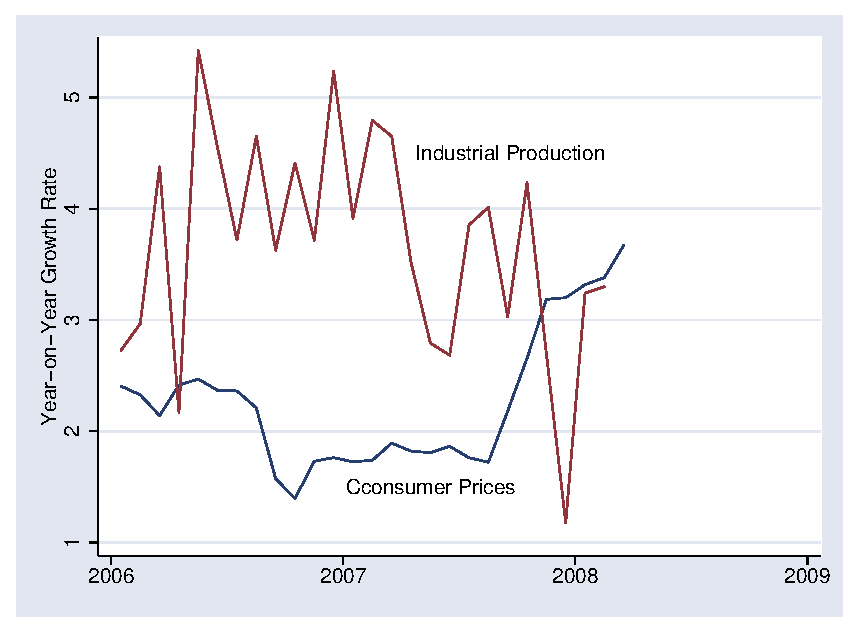
\includegraphics[scale=0.8]{final_08.eps}
    \caption{Growth in prices and industrial production in the
    Euro Zone.}
    \label{fig:ez}
\end{figure}

\item Aggregate supply and demand in the Euro Zone,
May 2008.
As the CFO of Heineken International, you are considering
the likely evolution of interest rates in the Euro Zone.
You quickly run through the following questions:
%
\begin{enumerate}

\item Over the 2-year period as a whole,
    what has happened to inflation and output?
    See Figure \ref{fig:ez};
    nothing is needed beyond what you see there.

\item In the aggregate supply and demand framework,
    do you think the movements in prices and output
    you mentioned above suggest a shift in supply or demand?  Why?
    In principle,
    how should the European Central Bank respond to such a shift?

\item How do you think the European Central Bank is
likely to respond?
How do you see short-term Euro Zone
interest rates moving over the next 12 months? Why?

\end{enumerate}


%\begin{comment}
Answer.
\begin{enumerate}
\item Inflation is up sharply, output is flat to down.

\item The combination in (a) suggests a shift up/left in supply.
Why?  Because output and inflation have moved in opposite directions.
Since supply shocks should be accommodated/reinforced,
the ECB should raise the short-term interest rate.

\item The ECB's primary mission is stable prices,
so you should see an increase in interest rates.
This could also be expressed in terms of a Taylor rule,
possibly with a larger coefficient on inflation
than output growth.
\end{enumerate}

\item Current economic conditions. 
\begin{enumerate}
\item  What have inflation and GDP growth been over the past quarter?  Year?
\item Using this information and anything else you think is appropriate, 
where is the economy relative to the long-run equilibrium level of output $Y^*$?  
\end{enumerate}
\end{enumerate}


\subsubsection*{If you're looking for more}

The measurement of potential output has generated some interesting debate.
Here is a range of opinion on the subject:
%
\begin{itemize}
\item Former Fed Governor Frederic Mishkin's
\href{http://www.federalreserve.gov/newsevents/speech/mishkin20070524a.htm}{speech}.

\item Robert Hall's
\href{http://www.kc.frb.org/publicat/Sympos/2005/PDF/Hall2005.pdf}{critique} of standard practice or
(better yet) Greg Mankiw's lucid and short
\href{http://www.kc.frb.org/publicat/Sympos/2005/PDF/Mankiw2005.pdf}{summary and discussion}.
The essence of Hall's argument is that potential output may very well not be smooth,
which would contradict most measures of it.
As a practical matter, this would change our view of monetary policy dramatically,
since many of the movements we see in GDP would be the result of the invisible hand,
and therefore not something for policymakers to offset.

\end{itemize}

\vfill \centerline{\it \copyright \ \number\year \ NYU Stern
School of Business}

\end{document}

\newpage
\subsubsection*{Multipliers}

?? ...

OLD STUFF

\subsubsection*{Beyond supply and demand}

Aggregate supply and demand is
how most textbooks treat business cycles.
It's also behind much of what you read in the business press.
But it's not how academic economists think about them.
The issue is dynamics:  there are no dynamics in the model.
And when you start thinking about dynamics,
some tricky issues come up that we've ignored ---
perhaps right so!
The central one is that current decisions typically depend
not only on current conditions, but
on what people expect conditions to be in the future.
That makes it difficult to determine causality:
did the present cause the future, or the reverse?


Think about popular comments to the effect that
consumer demand is driving the economy.
A journalist might say:  high consumer demand led to an economic boom.
The logic is perfectly consistent with our AS/AD analysis,
but is that really what's going on?
If we think about consumption,
one of our first thoughts should be to think about our future income.
If we expect to have much higher income in the future
(that MBA is really paying off!),
we might consume more now.
But think about what that does to causality:
for the economy as a whole, has output gone up because we consumed
more, or did we consume more because we expected output to go up?
It's not easy to tell the difference between the two arguments.


Investment is similar.  Firms make investment decisions
based on their assessment (ie, guess)
of market conditions years down the road.
That's why ``institutions'' are so important:
good institutions give firms some assurance that the rules won't change
in ways that make the investment less attractive.
With respect to business cycles, we could ask the same question
we asked of consumption:
did high investment lead to a booming economy,
or did expectations of a booming economy lead to high investment?
If we're forecasting, we may not care, as long as the two go
together.
But if we want to understand what's going on, we need to address
this issue one way or the other.
Fed minutes and analyst reports
are filled with conjectures over exactly this kind of issue.

Sticky wages are another example.
We noted that output may be below its long-run
level if the real wage is too high.
%:  if the wage rate is above where supply equals demand for labor.
But how was that wage set?
If workers and firms expect conditions to lead wages to be too high,
why don't they set a lower wage?
There may be reasons this could happen anyway,
but the point is that wages will be based, in part,
on expected future conditions.

%All of these examples suggest that the economy is more complicated
%than the aggregate supply and demand apparatus indicates.

